
%(BEGIN_QUESTION)
% Copyright 2012, Tony R. Kuphaldt, released under the Creative Commons Attribution License (v 1.0)
% This means you may do almost anything with this work of mine, so long as you give me proper credit

The mechanism of a high-voltage oil-tank circuit breaker is typically actuated by the power of compressed air in a double-acting cylinder:

$$\includegraphics[width=15.5cm]{i01213x01.eps}$$

Sketch the correct arrow symbols inside the spool valve's square symbols in order to make the breaker trip and close as those respective solenoid coils are energized.  The actuating cylinder needs to remain ``locked'' in position when neither solenoid coil is energized.

\vskip 10pt

Finally, identify the other pneumatic components in the system.

\vskip 20pt \vbox{\hrule \hbox{\strut \vrule{} {\bf Suggestions for Socratic discussion} \vrule} \hrule}

\begin{itemize}
\item{} Explain why the circuit breaker must be actuated by compressed air, rather than being directly actuated by solenoid coils.
\item{} Suppose the compressed air reliabilty (i.e. the probabilty there will be sufficient pressure and volume of compressed air for the breaker to actuate) has a rating of 0.992, the ``Close'' valve function has a dependability rating of 0.942, and the cylinder has a dependability rating of 0.9991.  From these ratings calculate the dependability of the breaker's ``close'' function.
\end{itemize}

\underbar{file i01213}
%(END_QUESTION)





%(BEGIN_ANSWER)


%(END_ANSWER)





%(BEGIN_NOTES)

$$\includegraphics[width=15.5cm]{i01213x02.eps}$$

%INDEX% Electric power systems: HV circuit breaker controls
%INDEX% Final Control Elements, valve: solenoid
%INDEX% Mechanics, fluid power systems: reversing (double-acting) cylinder control

%(END_NOTES)


